%% This is file `elsarticle-template-1-num.tex',
%%
%% Copyright 2009 Elsevier Ltd
%%
%% This file is part of the 'Elsarticle Bundle'.
%% ---------------------------------------------
%%
%% It may be distributed under the conditions of the LaTeX Project Public
%% License, either version 1.2 of this license or (at your option) any
%% later version.  The latest version of this license is in
%%    http://www.latex-project.org/lppl.txt
%% and version 1.2 or later is part of all distributions of LaTeX
%% version 1999/12/01 or later.
%%
%% The list of all files belonging to the 'Elsarticle Bundle' is
%% given in the file `manifest.txt'.
%%
%% Template article for Elsevier's document class `elsarticle'
%% with numbered style bibliographic references
%%
%% $Id: elsarticle-template-1-num.tex 149 2009-10-08 05:01:15Z rishi $
%% $URL: http://lenova.river-valley.com/svn/elsbst/trunk/elsarticle-template-1-num.tex $
%%
\documentclass[5p,12pt]{elsarticle}
\usepackage{amsmath}
\usepackage{graphicx,subcaption}
\usepackage{listings}
\usepackage{hyperref}
\usepackage{multirow}
\usepackage{notoccite}
\hypersetup{
    colorlinks,
    citecolor=black,
    filecolor=black,
    linkcolor=black,
    urlcolor=black
}

%% Use the option review to obtain double line spacing
%% \documentclass[preprint,review,12pt]{elsarticle}

%% Use the options 1p,twocolumn; 3p; 3p,twocolumn; 5p; or 5p,twocolumn
%% for a journal layout:
%% \documentclass[final,1p,times]{elsarticle}
%% \documentclass[final,1p,times,twocolumn]{elsarticle}
%% \documentclass[final,3p,times]{elsarticle}
%% \documentclass[final,3p,times,twocolumn]{elsarticle}
%% \documentclass[final,5p,times]{elsarticle}
%% \documentclass[final,5p,times,twocolumn]{elsarticle}

%% if you use PostScript figures in your article
%% use the graphics package for simple commands
%% \usepackage{graphics}
%% or use the graphicx package for more complicated commands
%% \usepackage{graphicx}
%% or use the epsfig package if you prefer to use the old commands
%% \usepackage{epsfig}

%% The amssymb package provides various useful mathematical symbols
\usepackage{amssymb}
%% The amsthm package provides extended theorem environments
%% \usepackage{amsthm}

%% The lineno packages adds line numbers. Start line numbering with
%% \begin{linenumbers}, end it with \end{linenumbers}. Or switch it on
%% for the whole article with \linenumbers after \end{frontmatter}.
\usepackage{lineno}
\usepackage{enumitem}

%% natbib.sty is loaded by default. However, natbib options can be
%% provided with \biboptions{...} command. Following options are
%% valid:

%%   round  -  round parentheses are used (default)
%%   square -  square brackets are used   [option]
%%   curly  -  curly braces are used      {option}
%%   angle  -  angle brackets are used    <option>
%%   semicolon  -  multiple citations separated by semi-colon
%%   colon  - same as semicolon, an earlier confusion
%%   comma  -  separated by comma
%%   numbers-  selects numerical citations
%%   super  -  numerical citations as superscripts
%%   sort   -  sorts multiple citations according to order in ref. list
%%   sort&compress   -  like sort, but also compresses numerical citations
%%   compress - compresses without sorting
%%
%% \biboptions{comma,round}

% \biboptions{}


%\makeatletter
%\providecommand{\doi}[1]{%
%  \begingroup
%    \let\bibinfo\@secondoftwo
%    \urlstyle{rm}%
%    \href{http://dx.doi.org/#1}{%
%      doi:\discretionary{}{}{}%
%      \nolinkurl{#1}%
%    }%
%  \endgroup
%}
%\makeatother

\let\originaleqref\eqref
\renewcommand{\eqref}{Eq.~\originaleqref}

\hypersetup{colorlinks=true,
  pdftitle={Neutron Brilliance of the Liquid Deuterium Cold Source as Measured from the ICON Beamline at the Swiss Spallation Neutron Source (SINQ)},
  pdfauthor={Ryan M. Bergmann, Masako Yamada, Tibor Reiss, Vadim Talanov, Michael Wohlmuther, Uwe Filges}}

\journal{Nuclear Instruments and Methods in Physics Research Section A: Accelerators, Spectrometers, Detectors and Associated Equipment}

\begin{document}

\begin{frontmatter}

%% Title, authors and addresses

%% use the tnoteref command within \title for footnotes;
%% use the tnotetext command for the associated footnote;
%% use the fnref command within \author or \address for footnotes;
%% use the fntext command for the associated footnote;
%% use the corref command within \author for corresponding author footnotes;
%% use the cortext command for the associated footnote;
%% use the ead command for the email address,
%% and the form \ead[url] for the home page:
%%
%% \title{Title\tnoteref{label1}}
%% \tnotetext[label1]{}
%% \author{Name\corref{cor1}\fnref{label2}}
%% \ead{email address}
%% \ead[url]{home page}
%% \fntext[label2]{}
%% \cortext[cor1]{}
%% \address{Address\fnref{label3}}
%% \fntext[label3]{}

\title{Neutron Brilliance of the Liquid Deuterium Cold Source as Measured from the ICON Beamline at the Swiss Spallation Neutron Source (SINQ)}

%% use optional labels to link authors explicitly to addresses:
%% \author[label1,label2]{<author name>}
%% \address[label1]{<address>}
%% \address[label2]{<address>}

\author[]{Ryan M. Bergmann\corref{cor1}}
\ead{ryan.bergmann@psi.ch}

\author[]{Masako Yamada\corref{cor2}}
\ead{masako.yamada@psi.ch}

\author[]{Uwe Filges}
%\ead{uwe.filges@psi.ch}

\author[]{Tibor Reiss}
%\ead{tibor.reiss@psi.ch}

\author[]{Vadim Talanov}
%\ead{vadim.talanov@psi.ch}

\author[]{Michael Wohlmuther}
%\ead{michael.wohlmuther@psi.ch}

\address{Paul Scherrer Institut, Villigen, Switzerland}

\cortext[cor1]{Primary corresponding author. Tel.: +41.56.310.56.12.}
\cortext[cor2]{Corresponding author. Tel.: +41.56.310.50.64.}

\begin{abstract}

A brilliance measurement was conducted on July 21, 2014 at the ICON beamline at SINQ as a benchmark before any potential changes are made to the liquid deuterium cold neutron source in a future extended shutdown period.  The peak brilliance of the deuterium cold source at SINQ has been measured to be $3.5 \pm 0.28\times10^{11}$ n cm$^{-2}$ s$^{-1}$ mA$^{-1}$ \AA$^{-1}$ str$^{-1}$ (8\%) at 1.9 {\AA}, and the total brilliance (energy-integrated) has been measured to be  $9.91 \pm 2.2\times10^{11}$  n cm$^{-2}$ s$^{-1}$ mA$^{-1}$ str$^{-1}$ for wavelengths above 0.7 {\AA} via a time-of-flight measurement at the ICON beamline.  Using a very detailed MCNP model, the peak brilliance has been calculated to be $3.1 \pm 0.14\times10^{11}$ n cm$^{-2}$ s$^{-1}$ mA$^{-1}$ \AA$^{-1}$ str$^{-1}$ (8\%) at 1.65 {\AA}, and the total brilliance (energy-integrated) has been calculated to be  $8.97 \pm 1.7\times10^{11}$  n cm$^{-2}$ s$^{-1}$ mA$^{-1}$ str$^{-1}$ for wavelengths above 0.7 {\AA}.

\end{abstract}

\begin{keyword}
spallation \sep neutron \sep source \sep brilliance \sep cold \sep deuterium \sep measurement \sep helium-3 \sep detector


\end{keyword}


\end{frontmatter}

%\linenumbers

%% main text

\section{Introduction}
\label{sec:intro}

The Swiss Spallation Neutron Source (SINQ) is a spallation neutron source driven by a continuous 590 MeV proton beam at the Paul Scherrer Institut in Villigen, Switzerland \cite{hipa}.  Inside SINQ, incoming protons impinge on a lead target cooled with heavy water, producing high energy neutrons.  These neutrons are moderated by the tank of room temperature D$_2$O surrounding the target.  Within the D$_2$O moderator tank, there is a 20 liter volume of approximately 25 K liquid D$_2$ whose innermost face is approximately 35 cm away from the center of the target.  This volume, the ``cold source'', serves to further reduce the energies of the ``thermal'' neutrons coming from the D$_2$O tank into a regime that is more useful to scientific instruments at SINQ.  

There is an extended shutdown of SINQ ambitiously planned for 2018 which will provide an opportunity for changes to be made to the cold neutron source and the neutron guides \cite{rueegg_icans}.  The brilliance measurement presented in this paper was conducted to provide a reference to compare to after the upgrade has been completed.  Several time-of-flight (TOF) neutron spectrum measurements were conducted on July 21, 2014 at the ICON beamline at SINQ to determine the brilliance of the cold source.  ICON is the cold neutron imaging facility at SINQ.  The beamline offers an aperture wheel to change beam intensity and collimation ratio, as well as large, evacuated flight tubes to minimize losses from scattering in the air \cite{icon}.  ICON was chosen for the measurement since it does not incorporate any neutron optics, has good collimation, and looks directly on the surface of the cold source.  Measuring at ICON removes additional uncertainty associated with the current state of the neutron guides, eliminates having to model additional physics involved with neutron-reflective surfaces, and limits the detector view in a well-defined way.


%
%
%
%
%


\section{Experimental Setup}
\label{sec:setup}

The layout of the experiment is shown in Figure \ref{fig:geom} as a horizontal cut of the MCNP model geometry.  The target and moderators are shown furthest to the right.  The vertical line is the shielding monolith boundary, which is mostly steel blocks.  The ICON bunker is to the left of the monolith, the walls of which are made of heavy concrete and are shown as rectangular blocks.  The velocity selector that is usually mounted on the monolith wall in the ICON bunker was removed for this measurement.  A large number of shielding elements were used in this measurement since there is a large fast neutron background present at the ICON beamline.

\begin{figure*}[ht!] 
  \centering
    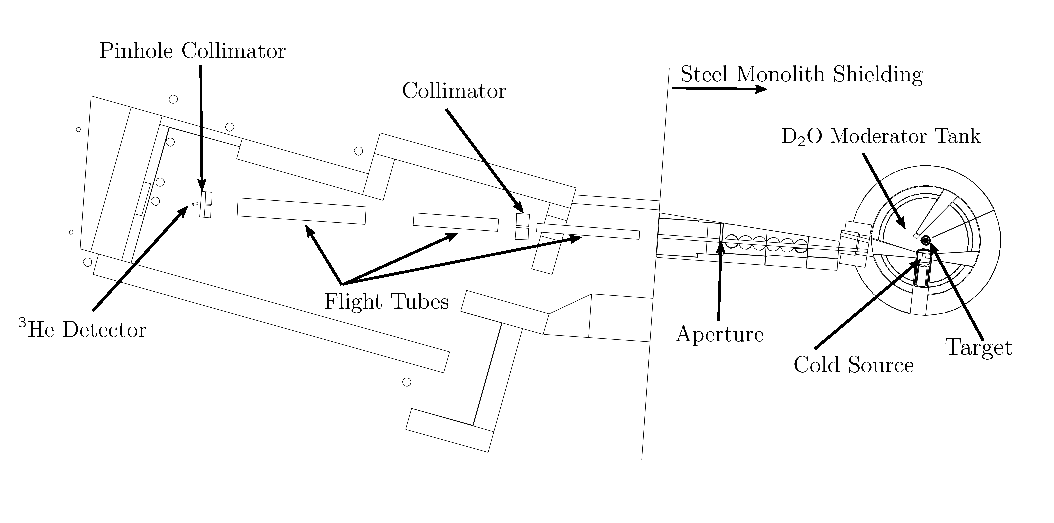
\includegraphics[width=0.9\textwidth]{graphics/geom_bw_labels.eps}
     \caption{A horizontal cut through the MCNP simulation geometry showing the major items in the neutron path. \label{fig:geom} }
\end{figure*}

Figure \ref{fig:det} shows a photograph of the $^3$He detector used in the TOF measurements with the iron pinhole collimator positioned in front of it.   This picture was taken before the large shielding blocks and sapphire crystals were positioned around the detector.

\begin{figure}[h!] 
  \centering
    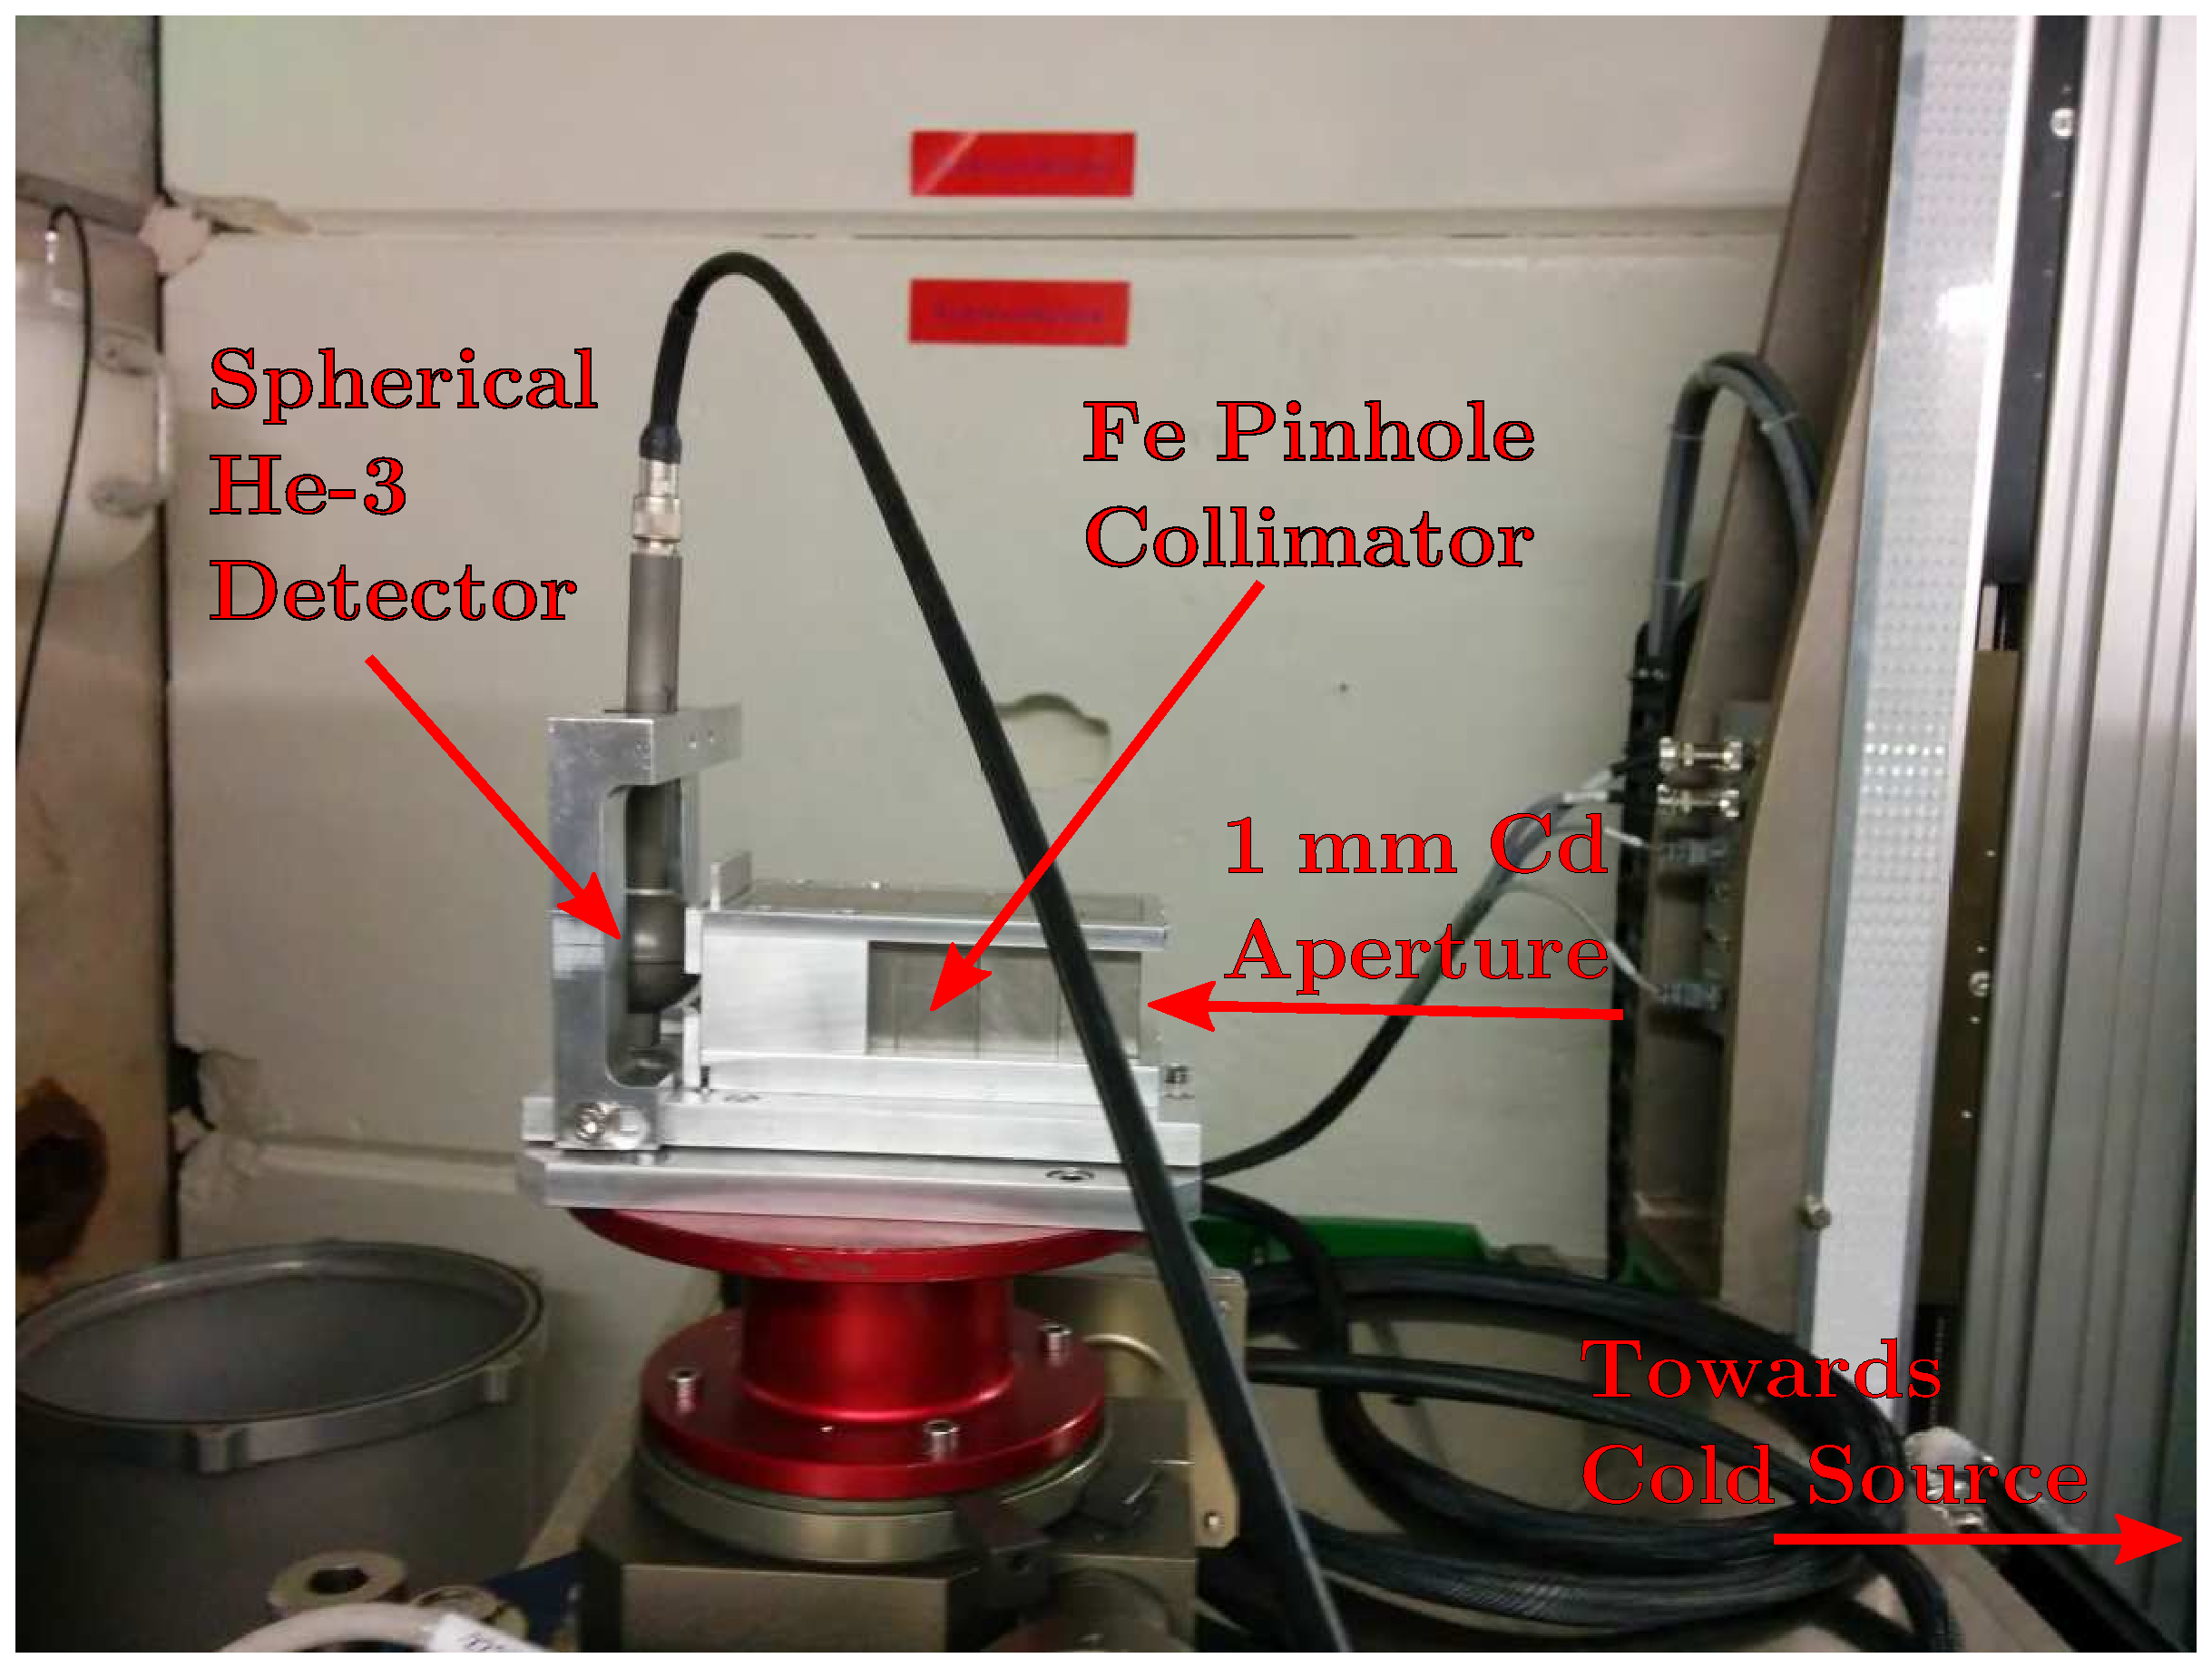
\includegraphics[width=\columnwidth]{graphics/det.eps}
     \caption{$^3$He detector with iron collimator. \label{fig:det}}
\end{figure}

The principle components in the neutron path, in order of increasing distance from the detector during the measurement, are shown in the following list.

\begin{center} \underline{In-bunker components}\end{center}
\begin{enumerate}
  \item Spherical $^3$He detector, 3.30 cm $\oslash$ gas volume, 0.5 mm thick stainless steel walls, surrounded by 1 mm cadmium sheets on all sides except towards the pinhole collimator
  \item Cadmium aperture, 1 mm $\oslash$ hole, 1 mm thick, 1 mm from the detector surface
  \item Iron pinhole collimator, 2 mm $\oslash$ hole, 100 mm long, immediately after the cadmium aperture, surrounded by heavy concrete, lead, and polyethylene shielding
  \item Sapphire crystals, 20x20 mm faces, 80 mm total thickness, within the heavy concrete, lead, and polyethylene shielding
  \item Three evacuated flight tubes with 1.0 mm thick aluminum windows, ~7410 mm total length, decreasing $\oslash$ of 41 cm, 30 cm, and 20 cm as distance to the source decreases. 
  \item Neutron chopper, Al-clad Cd, 420 mm $\oslash$ wheel, 1.5 mm thick, 30 Hz rotation speed, 7452 mm from the $^3$He detector, 2 mm wide slit corresponding to a 16\% duty cycle
  \item Steel collimator, 50x50 mm aperture, 30 cm thick, 7548 mm from detector
\end{enumerate}
\begin{center}\underline{In-pile components}\end{center}
\begin{enumerate}[resume]
  \item Movable gadolinium circular aperture wheel, set to the largest opening of 80 mm $\oslash$
  \item High energy shutters
  \item ``Zapfen'' unit, 40x120 mm
  \item D$_2$O moderator tank
  \item Low pressure nozzle which penetrates the D$_2$O moderator tank, opening size is approximatel 138x138 mm at the cold source surface
  \item Liquid deuterium cold source
  \item Lead ``cannelloni'' spallation target
\end{enumerate}


Since brilliance was the goal of the measurement, the solid angle seen by the detector was needed to normalize the neutron spectra.  The cadmium aperture limits the sensitive region of the helium detector to a 1 mm diameter circle, and the other items in the beam path created a system that limited the angular view of the detector.  Table \ref{tab:sa} shows the maximum solid angle of the various items in the neutron beam (i.e the penumbra created by these objects).  The values are the minima of the item's self-collimation (due to its thickness) and the collimation of the system formed by the item and the hole in the cadmium sheet.  Figure \ref{fig:solid_angle} shows a cartoon of the collimation system formed by the items and the cadmium hole.  It can be seen that in the horizontal plane, the Zapfen opening (where the beamline opens into large nozzle in the moderator tank) is the limiting item.  In the vertical plane, the limiting item is the beam tube between the Zapfen and the monolith wall.  At 45 degrees of azimuthal angle, the aperture wheel is the limiting case.  These items are shown in the pinhole image calculated with MCNP and discussed in Section \ref{sec:sim}.

\begin{figure}[h!] 
  \centering
    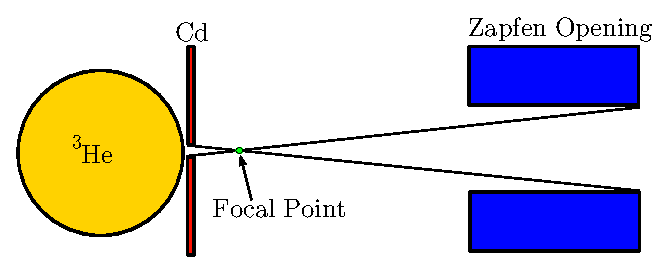
\includegraphics[width=\columnwidth]{graphics/solid_angle.eps}
     \caption{The limiting collimation system in the measurement in the horizontal plane (not to scale), and the crossing point where the point detector was place in the MCNP simulations. \label{fig:solid_angle}}
\end{figure}

\begin{table}
\scriptsize
\begin{center}
     \caption{Table of solid angles with the limiting member marked with boldface and a star (*).  \label{tab:sa} }
\begin{tabular}{|l|r|r|r|}
     \hline
                   &     Horizontal  &     Vertical   &     Diagonal   \\
     \hline
     Fe Collimator &     6.93E-4  &     6.93E-4 &     6.93E-4 \\
     \hline 
     Cadmium Hole  &     1.84E-0  &     1.84E-0 &     1.84E-0 \\
     \hline 
     Sapphire      &     1.98E-3  &     1.98E-3 &     3.84E-3 \\
     \hline 
     Steel         &     3.32E-5  &     3.32E-5 &     6.56E-5 \\
     \hline
     Aperture      &     3.40E-5  &     3.40E-5 &\bf* 3.40E-5 \\
     \hline
     Tube          &     2.26E-5  &\bf* 2.26E-5 &     4.49E-5  \\
     \hline
     Zapfen        &\bf* 2.07E-5  &     4.62E-5 &     6.66E-5 \\
     \hline
     Nozzle        &     5.13E-5  &     5.13E-5 &     1.02E-4 \\
     \hline
\end{tabular}
\end{center}
\end{table}

Three measurements were done in total: centered in the beam with sapphire crystals inside the nearest shielding, centered with a beryllium crystal cooled below 120 K (under which transmission does not change much) in the beamline to show the 4 {\AA} bin of the analyzer, and centered in the beam without sapphire or beryllium.  The center of the beam was found by scanning a neutron-sensitive CCD camera (which has layers of iron and cadmium before the CCD) through the beam and assuming the flux maximum was the beam center.  Once positioned at the center, the vertical tilt of the detector/pinhole system was scanned to find the maximum once again.  Since a measurement was not done with the shutter closed to collect background, the average value of lower-energy tail of the measured spectrum between 9.6 and 11.0 {\AA} was assumed to be the background level.

Since the viewing angle was wide for this measurement, it should be insensitive to variations introduced by alignment.  The detector saw almost the entire surface of the could source during the measurement, so moving it to the left or right in space should have produced similar intensiities as long as a new structure did not occlude the view.  Because of this wide view, there is little uncertainty on which region of the cold source the detector saw.   In other words, spectral variations between measured and calculated values should not be because the detector was similated with a different view of the cold source compared to what was measured.

%
%
%
%
%

%
%
%
%
%


\section{Detector Efficiency}
\label{sec:eff}

The efficiency curve of the helium detector was also measured and compared to calculated curves.  Curves were calculated using a one-dimensional (1D) model and 1/v cross sections as well as with a detailed MCNP model of the helium detector \cite{bonner_manual}.  The 1D model efficiency is shown in Eq. \ref{eqn:eff1}, where $\Sigma_{\textrm{stl}}$ is the stainless steel macroscopic total cross section, $\Sigma_{\textrm{He}}$ is the $^3$He macroscopic absorbtion cross section, $x_{\textrm{stl}}$ is the thickness of the detector's stainless steel shell, and  $D_{\textrm{He}}$ is the diameter $^3$He volume.  Since the beam is collimated by the cadmium aperture, it can be assumed that all neutrons pass through the center of the detector, and the problem can be approximated well as a 1-D system.  The cross section wavelength dependence is shown in Eq. \ref{eqn:eff2}, where $a$ and $b$ are linear fit coefficients derived from cross section data.  In this case, $b$ was set to zero and $a$ was set to the thermal absorption cross section ($\Sigma_{\textrm{abs}}$) multiplied by the number density of nuclei ($N$) with a proportionality constant of 1.8 so the cross section scales correctly with wavelength.

\begin{gather}
     \label{eqn:eff1} \epsilon(\lambda) = \exp \left(-\Sigma_{\textrm{stl}}(\lambda) x_{\textrm{stl}}\right)[1-\exp(-\Sigma_{\textrm{He}}(\lambda) D_{\textrm{He}})] \\
     \label{eqn:eff2} \Sigma_i(\lambda) = a_i\lambda+b_i  \sim  \frac{\Sigma_{\textrm{abs}}}{1.8} N \lambda 
\end{gather}

The efficiency curve was calculated from the MCNP model by directing a stream of neutrons in a 0.5 mm radius with a flat spectrum towards the midplane of the spherical detector, tallying the absorption reaction rate in $^{3}$He (which is the charge production rate in the detector volume), then dividing the absorption rate by the incoming source spectrum.  

The measured efficiency curve was taken at the BOA beamline at SINQ.  This was done by comparing the detector to another detector with a well-know efficiency (also a $^3$He detector).  The measured response of the helium sphere detector was divided by the measured spectrum  from the well-known detector to give the efficiency of the helium sphere detector.

Figure \ref{fig:eff} shows the two calculated efficiency curves against the measured curve.  The MCNP curve agrees very well with the measured curve, and was used to produce the measured brilliance spectrum in Section \ref{sec:results} since it is much less noisy than the measured curve.

\begin{figure}[h!] 
  \centering
    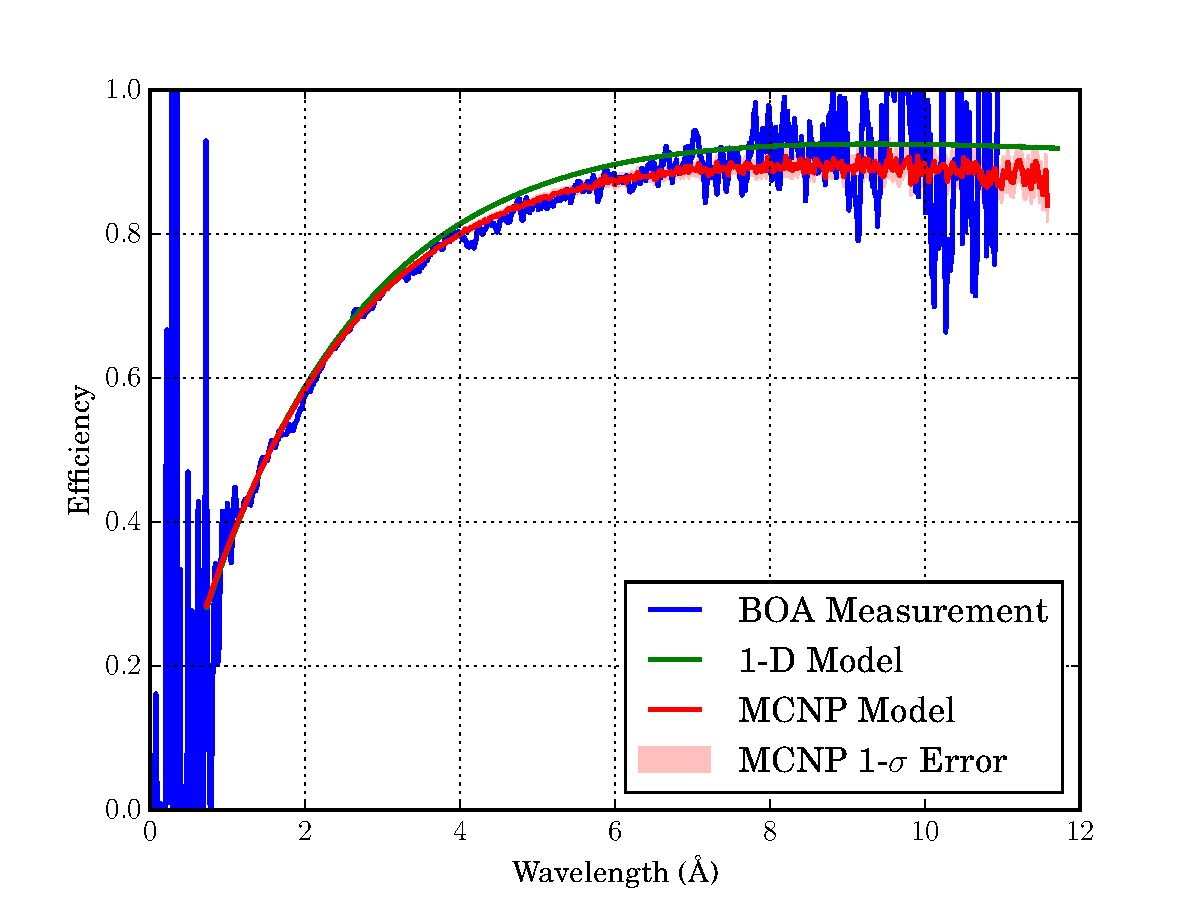
\includegraphics[width=\columnwidth]{graphics/eff.pdf}
     \caption{The efficiency curves. \label{fig:eff} }
\end{figure}


\section{Monte Carlo Simulations}
\label{sec:sim}

Simulations were done with MCNP6.1 and with ENDF/B-VII.1 data.  Thermal scattering data for the room temperature sapphire crystals were used \cite{sapp}, as were 77 K thermal scattering data for beryllium, various data for ortho-/para-deuterium, 273 K data for heavy water, 273 K data for light water \cite{mcnp6}, and 293 K data for aluminum, and 25 K data for zirconium \cite{IKE}.  The aluminum and zirconium data are important for accurately simulating the transmission through the various hulls surrounding the deuterium in the cold source.  The overall model geometry has already been shown in Figure \ref{fig:geom}, and was created to be as true-to-life as possible with very high levels of detail in the cold source and cannelloni target.  The detailed plot of the cold source geometry is shown on the right side of Figure \ref{fig:target}.  The cannelloni target in use during the measurement was ``target 10'', which is shown in left side of Figure \ref{fig:target}. This target had a hemispherical beam entrance window and ``SINQ Target Irradiation Program'' (STIP) material irradiation samples within the target.  Both of these features reduce the neutron flux compared to the highest performing target and were modelled in the MCNP simulation.

\begin{figure}[h!] 
  \centering
    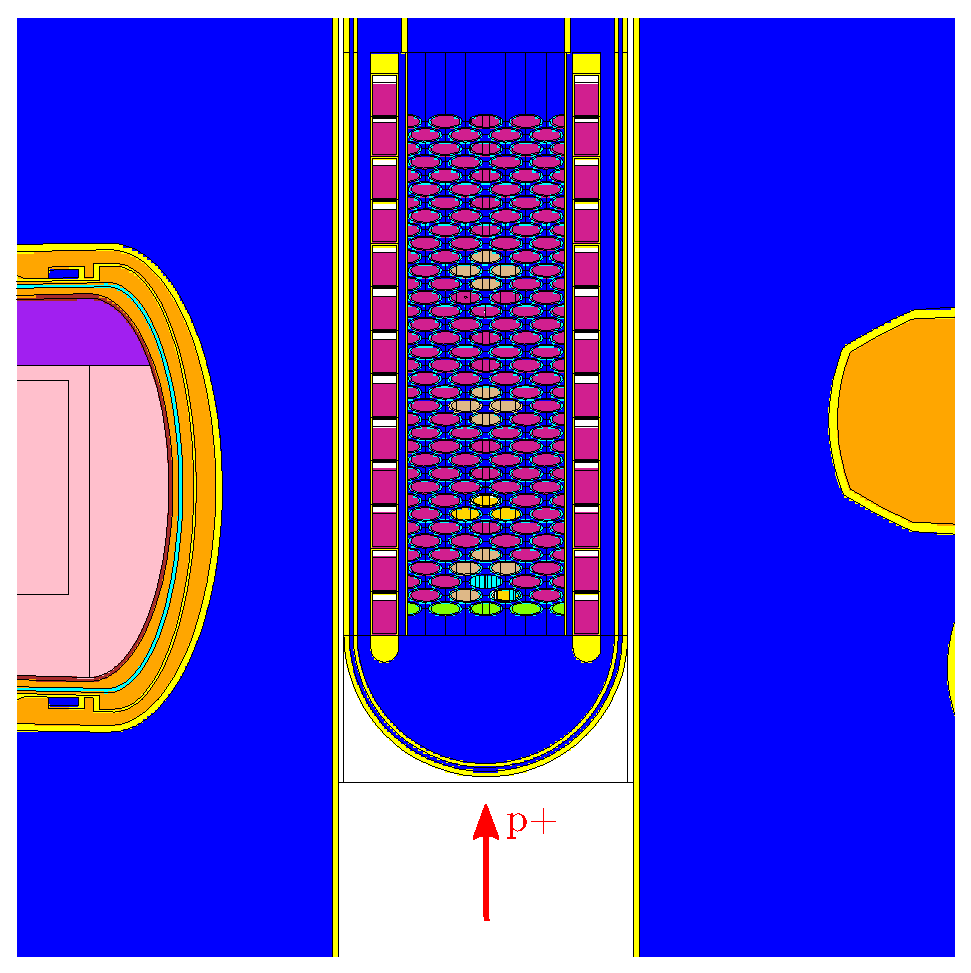
\includegraphics[width=0.25\columnwidth,trim={5cm 1cm 5cm 0cm},clip]{graphics/target.eps}
    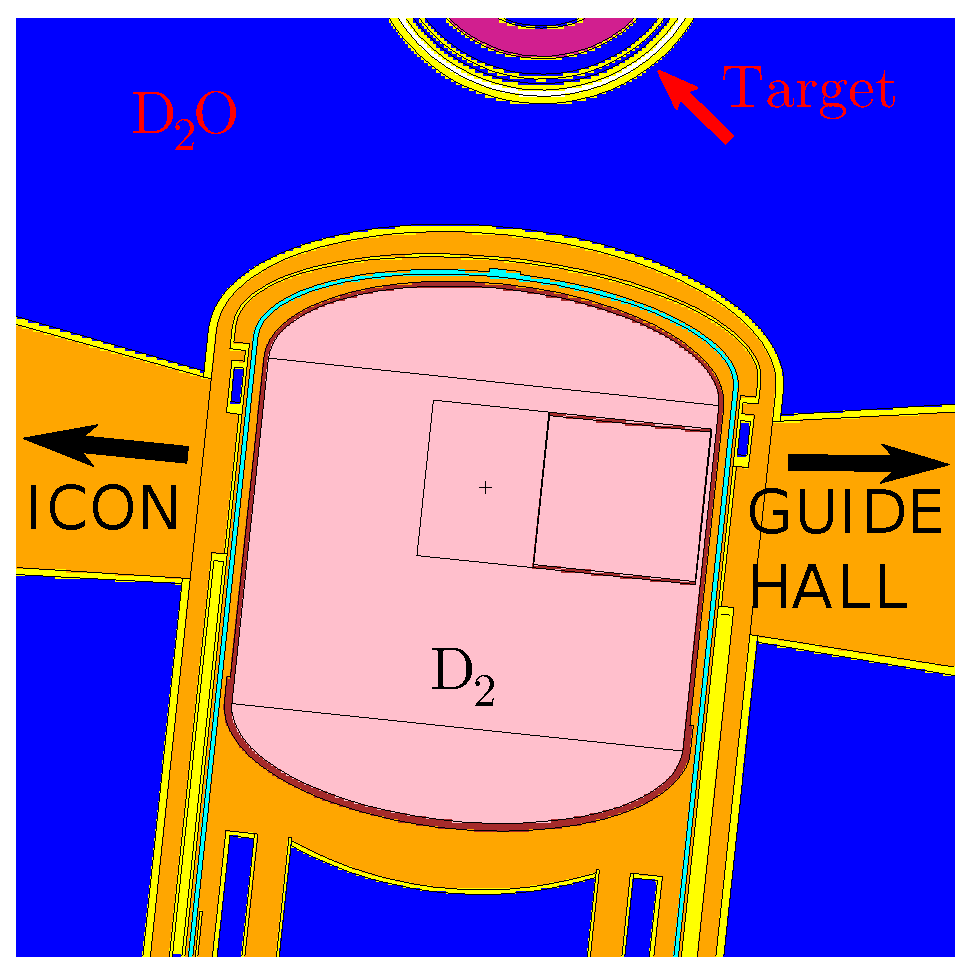
\includegraphics[width=0.63\columnwidth,trim={0cm 0cm 0cm 0cm},clip]{graphics/cs_xy.eps}
     \caption{LEFT: Vertical cross section of the cannelloni target geometry.  RIGHT:  Horizontal cross section of the cold source geometry of the MCNP model. The STIP samples are visible in the target model as brown, yellow, and blue rods.  The magenta colored rods in the target are filled with lead. \label{fig:target}}
\end{figure}

%
%
%
%
%

\subsection{Solid Angle Calculation}
\label{subsec:solidangle}

Since the detector is very far away from the neutron source, special methods had to be used in order to gather sufficient statistics in a reasonable amount of time.  A point detector is a ``next event'' estimator that calculates tally contributions at every neutron collision event \cite{mcnp5}.  The contribution to the tally is weighted by the probability of the neutron scattering into the direction of the detector point and travelling to the detector without colliding again (i.e. weight is reduced by the attenuation of the material in-between the scatter event and the detector position).  

Using a point detector would be a reasonable solution if only the calculated flux was desired, but the brilliance also depends on the viewable solid angle of the detector system.   The physical system responds to a view limited by the beamline components and cadmium aperture, and a regular point detector would integrate all visible contributions and wouldn't report any angular information needed for calculating the brilliance.  In order to calculate the solid angle visible to the $^3$He detector, a ``pinhole radiography tally'' was used in MCNP.  This tally calculates contributions the same way as a point detector, but it projects the contributions through the pinhole point onto a pre-defined image plane.  If such a pinhole detector is placed behind all the items which limit the detector view, the solid angle visible to the $^3$He detector can be calculated by summing the individual solid angle values each pixel of the pinhole image corresponds to.

Figure \ref{fig:pinhole_image} shows a pinhole radiography tally image generated at the upstream surface of the cadmium sheet with the pinhole placed at the horizontal collimation crossing point.  The Zapfen limits the view on the horizontal plane, so the hole in the cadmium (grey) lines up with projection of the Zapfen (magenta).  The other limiting objects are also projected onto the image plane in Figure \ref{fig:pinhole_image} to show the areas where they limit the detector view. The projections from the limiting objects are shown as dashed colored lines.   

\begin{figure}[h!] 
  \centering
    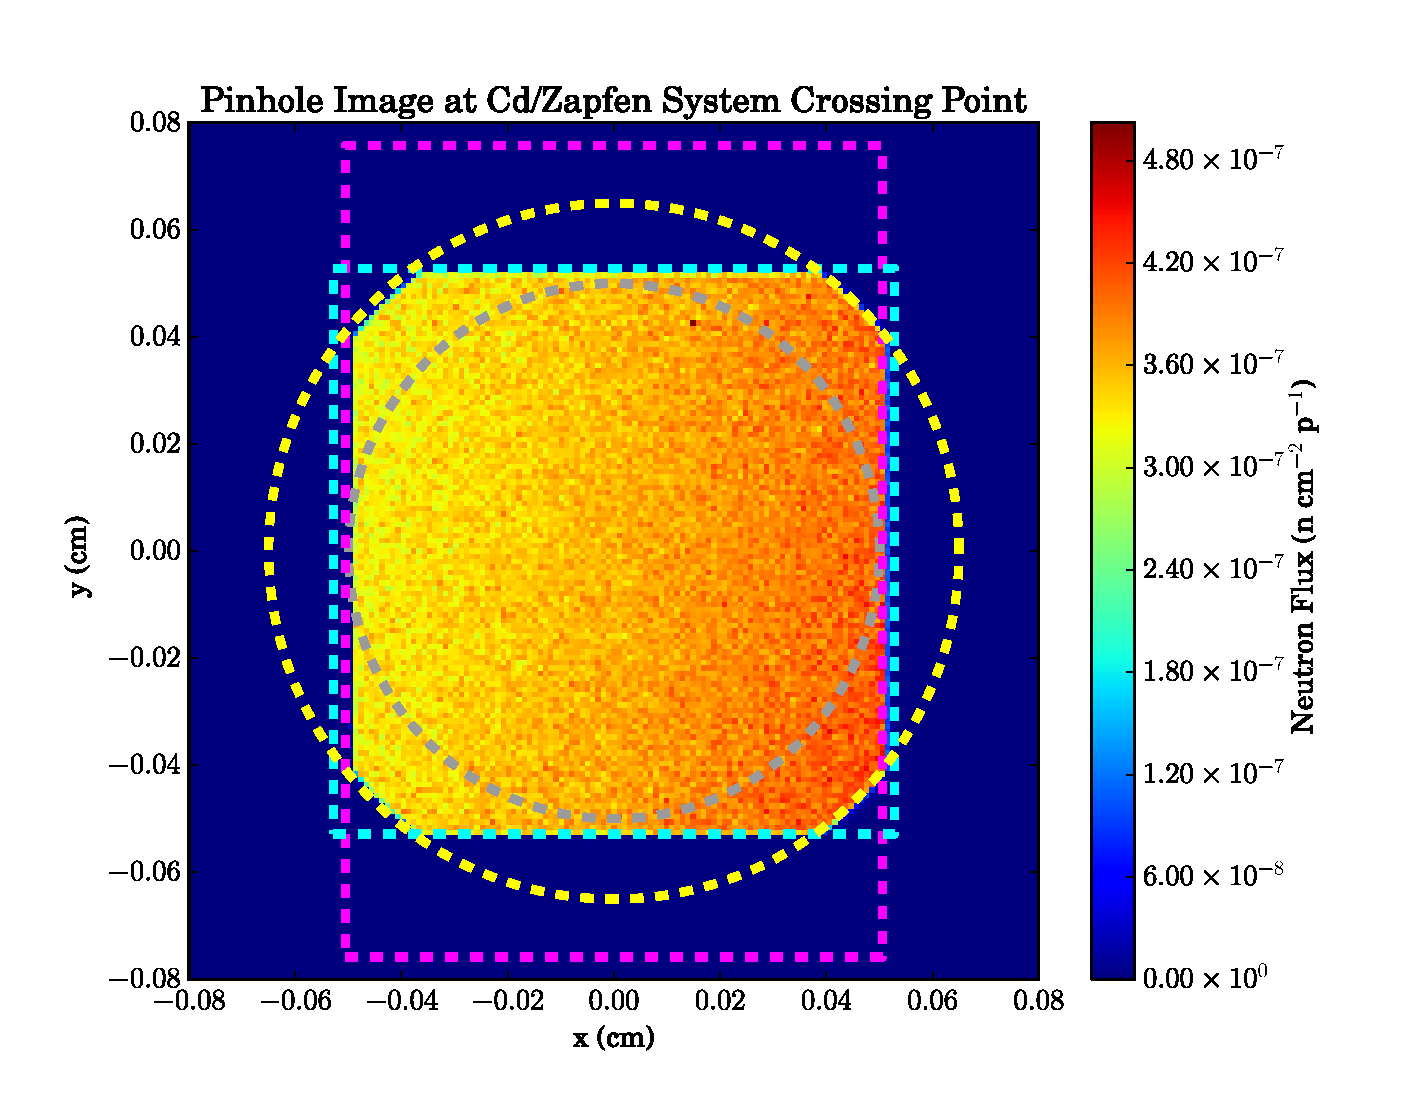
\includegraphics[width=\columnwidth]{graphics/pinhole.eps}
     \caption{The flux image created by a pinhole radiography tally in MCNP at the horizontal collimation crossing point.  The image plane is at upstream surface of the cadmium sheet.  The outlines show the projections of the limiting geometry through the pinhole: Grey=cadmium hole, blue=beam port, magenta=Zapfen, yellow=Gd aperture.  Note, the flux values shown are those resulting from a pinhole-limited view (not the real, full view).  \label{fig:pinhole_image}}
\end{figure}

The Zapfen is indeed the limiting member in the horizontal plane of the collimation system since it can be seen that the image does not extend past the magenta Zapfen projection line.  A horizontal and vertical gradient is also apparent in the projected image.  Since the dimensions are mirrored and the image is plotted from the view point of the pinhole towards the Cd sheet, the target would be to the right in the image and thermal flux maximum would be in the downward direction.

From this image, it was deduced that the total solid angle visible to the detector was limited to $2.1355\times10^{-5}$ steradians.  The hole is fully illuminated (there are no spots on the Cd sheet where a radiography tally produced a zero result), so the area used to normalize the spectra is simply the area of the hole (7.85398$\times 10^{-3}$ cm$^2$).  This value was used to normalize both the calculated and measured spectra, and therefore was not a source of uncertainty between the two.  

%
%
%
%
%

\subsection{Sensitivity to Scattering Data}
\label{subsec:data}

To calculate an accurate neutron spectrum emitted from the liquid deuterium in the cold source at low energies, thermal scattering data must be used to account for the influence of molecular bonds, crystal structure, nuclear alignment, etc.   There were several data libraries available when doing these MCNP calculations.  Namely, the default libraries from the ENDF/B-VII.1 data \cite{mcnp6}, several libraries from the Institut f\"{u}r Kernenergetik und Energiesysteme (IKE) at Universit\"{a}t Stuttgart \cite{IKE}, and those published by Centro At\'{o}mico Bariloche (CAB) \cite{granada_d2}.  The spectra calculated at the $^3$He detector position using the various liquid D$_2$ data are shown in Figure \ref{fig:data_compare_d2}.  It can be seen that the 24 K IKE data produce a significantly different spectrum compared to the ENDF 19 K data.  The 19 K CAB data also produce a significantly different spectrum compared to that produced with the 19 K ENDF data.  Since the effects are relatively large, the 24 K IKE data was chosen for the final simulation since it is nearest to the true temperature of the cold source.

\begin{figure}[h!] 
  \centering
    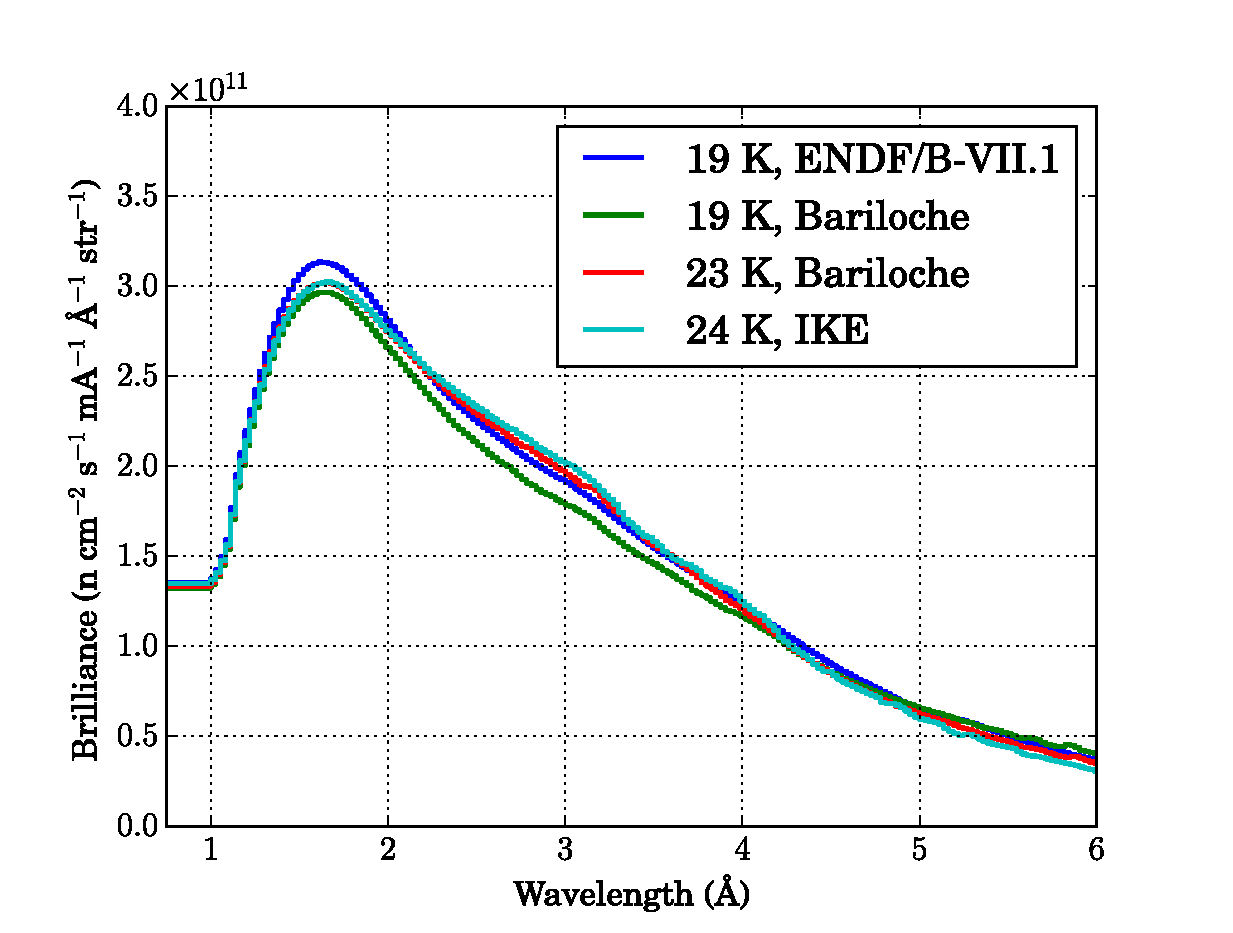
\includegraphics[width=\columnwidth]{graphics/data_compare_d2.eps}
     \caption{Simulated neutron spectra emitted from liquid deuterium cold source using various S($\alpha$,$\beta$) scattering data for D$_2$. \label{fig:data_compare_d2}}
\end{figure}  

Bariloche also released improved thermal scattering data for light and heavy water as well \cite{granada_d2o_1,granada_d2o_2,granada_d2o_3}.  The effect of replacing the ENDF/B-VII.1 data with the CAB data for both light and heavy water in the SINQ tank are shown in Figure \ref{fig:data_compare_d2o} when the standard D$_2$ scattering data and with liquid deuterium at 25 K  saturation density and long-time, 1.2 mA equilibrium o-D$_2$ fraction.  The figure shows that the updated heavy water data has very little effect on the emitted neutron spectrum from the cold source.  Therefore, the standard ENDF/B-VII.1 data was used in the final calculations, and this variation was not considered to be an uncertainty in the final calculated result.

\begin{figure}[h!] 
  \centering
    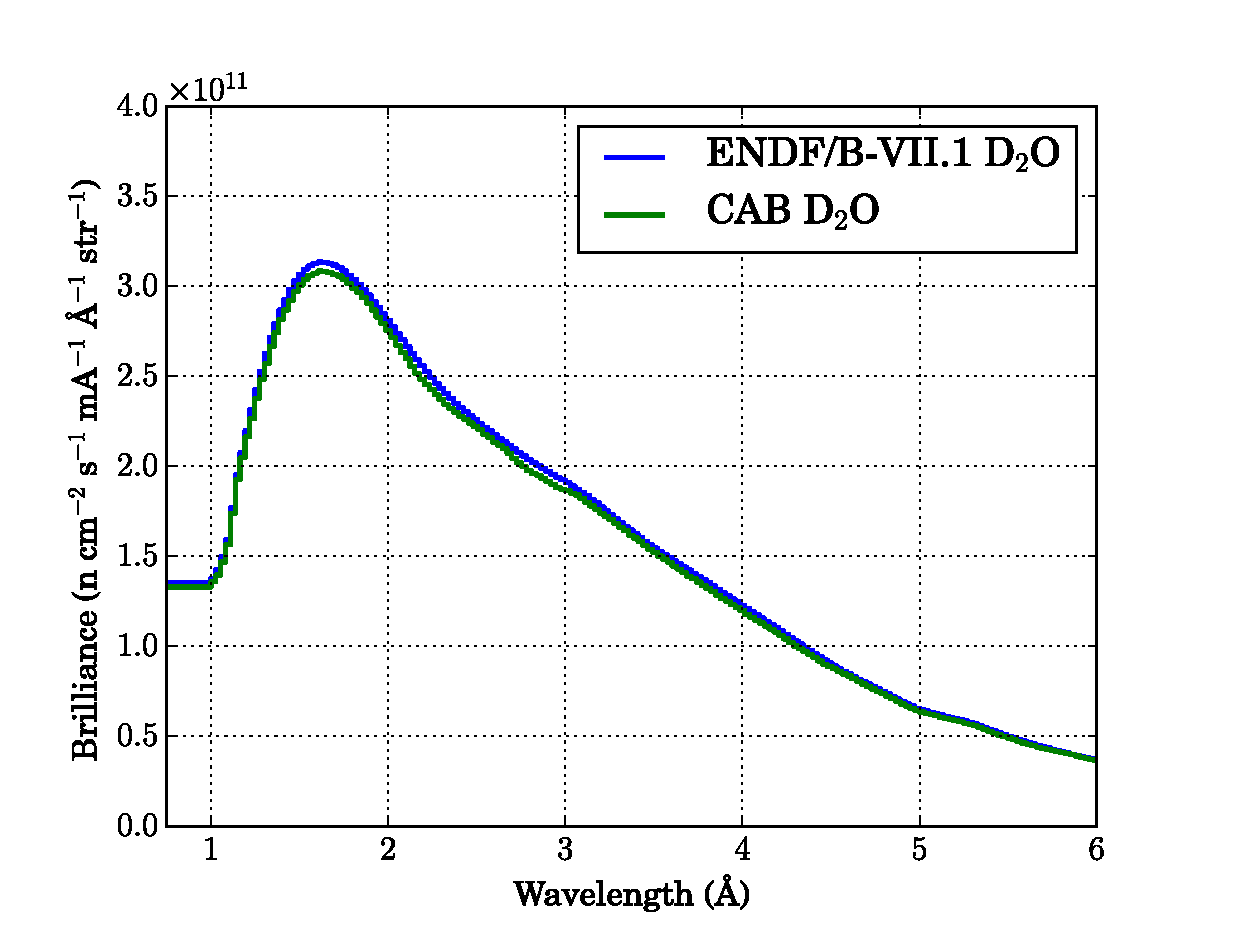
\includegraphics[width=\columnwidth]{graphics/data_compare_d2o.eps}
     \caption{Simulated neutron spectra emitted from liquid deuterium cold source using the standard ENDF/B-VII.1 and the new Bariloche S($\alpha$,$\beta$) scattering data for the D$_2$O moderator.   \label{fig:data_compare_d2o}}
\end{figure}

%
%
%
%
%

\subsection{Sensitivity to Ortho-/Para-D$_2$ Fraction and D$_2$ Density}
\label{subsec:frac_den}

Other than the data themselves, the spectrum emitted from the cold source is also sensitive to the density and the ortho- and para-D$_2$ fractions of the liquid deuterium.  These parameters effect the scattering length as well as the scattering kinematics of the moderator.  From the operational experience at the Institut Laue-Langevin (ILL), their 20 $\ell$ liquid deuterium cold source runs at about 80\% nominal density at 25 K at full reactor power \cite{ill_cns}. The nominal saturation density of liquid deuterium at 25 K is 0.162 g/cm$^3$\cite{bnl_cryo}.  Figure \ref{fig:density_compare} shows the variation of the neutrion spectrum due to density reduction from boiling in the deuterium.  A reduction of 80\% was chosen to be the maximum limiting case since the power deposition in the ILL cold source should be greater than that deposited in the SINQ deuterium volume.

\begin{figure}[h!] 
  \centering
    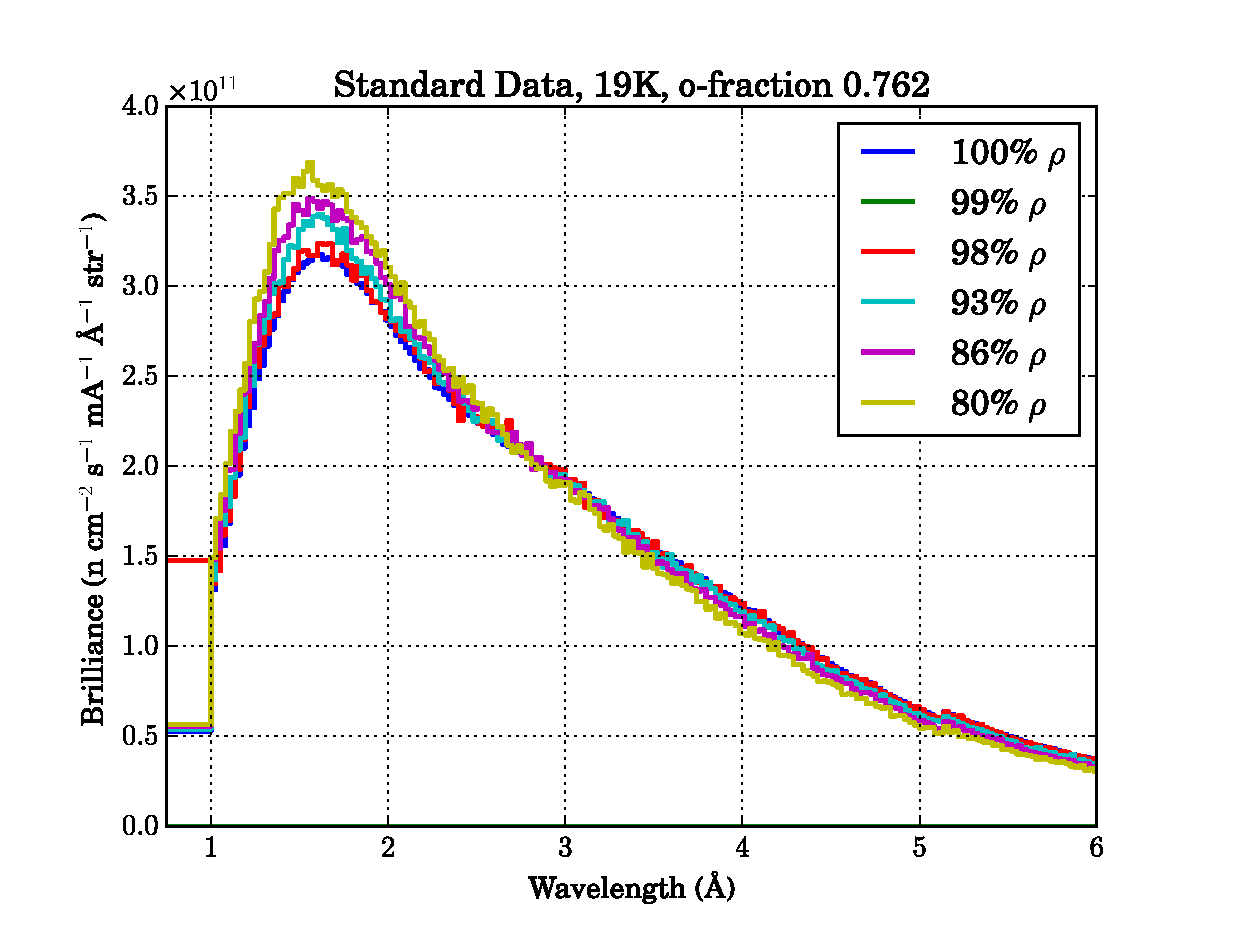
\includegraphics[width=\columnwidth]{graphics/density_compare.eps}
     \caption{Simulated neutron spectra emitted from liquid deuterium cold source at various D$_2$ densities. ENDFB/VII.1 19 K scattering data and a o-D$_2$ fraction of 0.762 was used.   \label{fig:density_compare}}
\end{figure}

Figure \ref{fig:density_compare} shows that the peak of calculated spectrum increases with density reduction.  Since the deuterium is more transparent to neutrons at lower densities, the emission region of the moderator becomes larger and less cold, increasing the thermal peak of the spectrum and reducing the cold region (wavelengths greater than the crossing point at 2.75 {\AA}).  From the MCNP simulations done, reducing the deuterium to 80\% nominal density (0.130 g/cm$^3$) increases thermal peak by about 12\%.

With no other influences, the thermodynamic equilibrium fraction of ortho-D$_2$ at 25 K is 0.955, but radiation-induced recombination of the deuterium molecules results in an equilibrium ratio of 0.762 for 1.2 mA of proton current on the SINQ target \cite{op_equi}.  This ratio gradually returns to thermodynamic equilibrium when the beam is shut off.  The proton current on SINQ prior to the brilliance measurement is shown in bottom plot in Figure \ref{fig:p_current}.  The was a relatively steady period of 1.5 mA for 13 weeks, with a service period of zero current of 1 week about 6 weeks before the measurement was taken.  The ortho-D$_2$ fraction was calculated based on this proton current history using the methods described in \cite{op_equi}, which accounts for the irradiation induced recombination, thermal conversion, catalytic conversion, and conversion from free atom collisions.  The results of the calculation are shown in upper plot in Figure \ref{fig:p_current}, with an initial ortho/para fraction of 2/3 (the room temperature, ``bottle'' equilibrium) after the shutdown period which ended May 1, 2014.  Figure \ref{fig:p_current} suggests the o-D$_2$ fraction during the measurement on July 21 should have been around 0.761.

\begin{figure}[h!] 
  \centering
    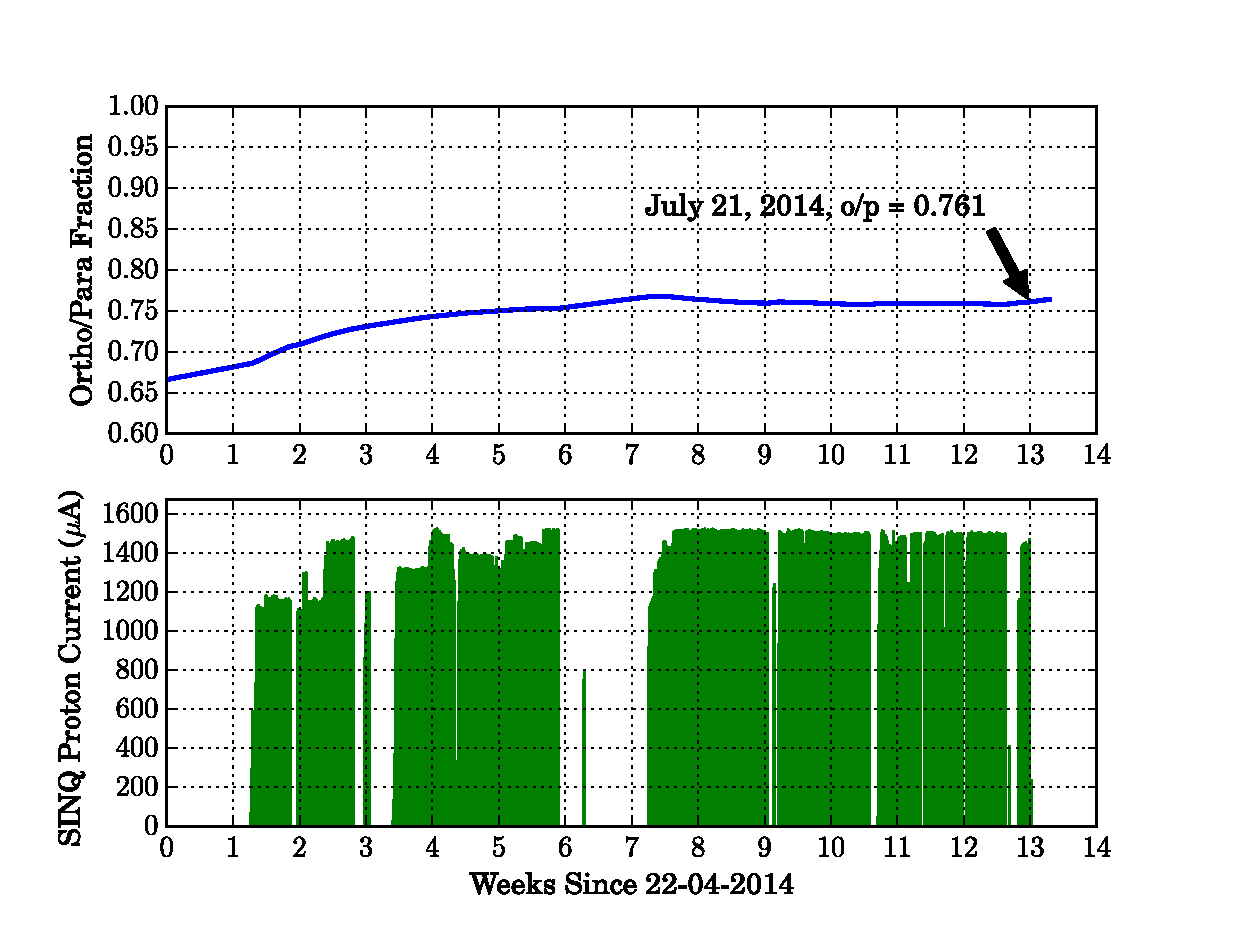
\includegraphics[width=\columnwidth]{graphics/p_current.eps}
     \caption{The proton current history for SINQ in the weeks leading up to the measurement time. \label{fig:p_current}}
\end{figure}

There is some uncertainty in this value, however, and Figure \ref{fig:op_compare} shows the variation in the emitted neutron spectrum caused by changing the o/p ratio in a range of 0.66 to 0.955 when the deuterium is at the 25 K saturation density of 0.162 g/cm$^3$ \cite{bnl_cryo}.  It is apparent that higher ortho fractions produce spectra with reduced neutron density at the thermal peak and enhanced density in cold regions $>$3.75 {\AA}.

\begin{figure}[h!] 
  \centering
    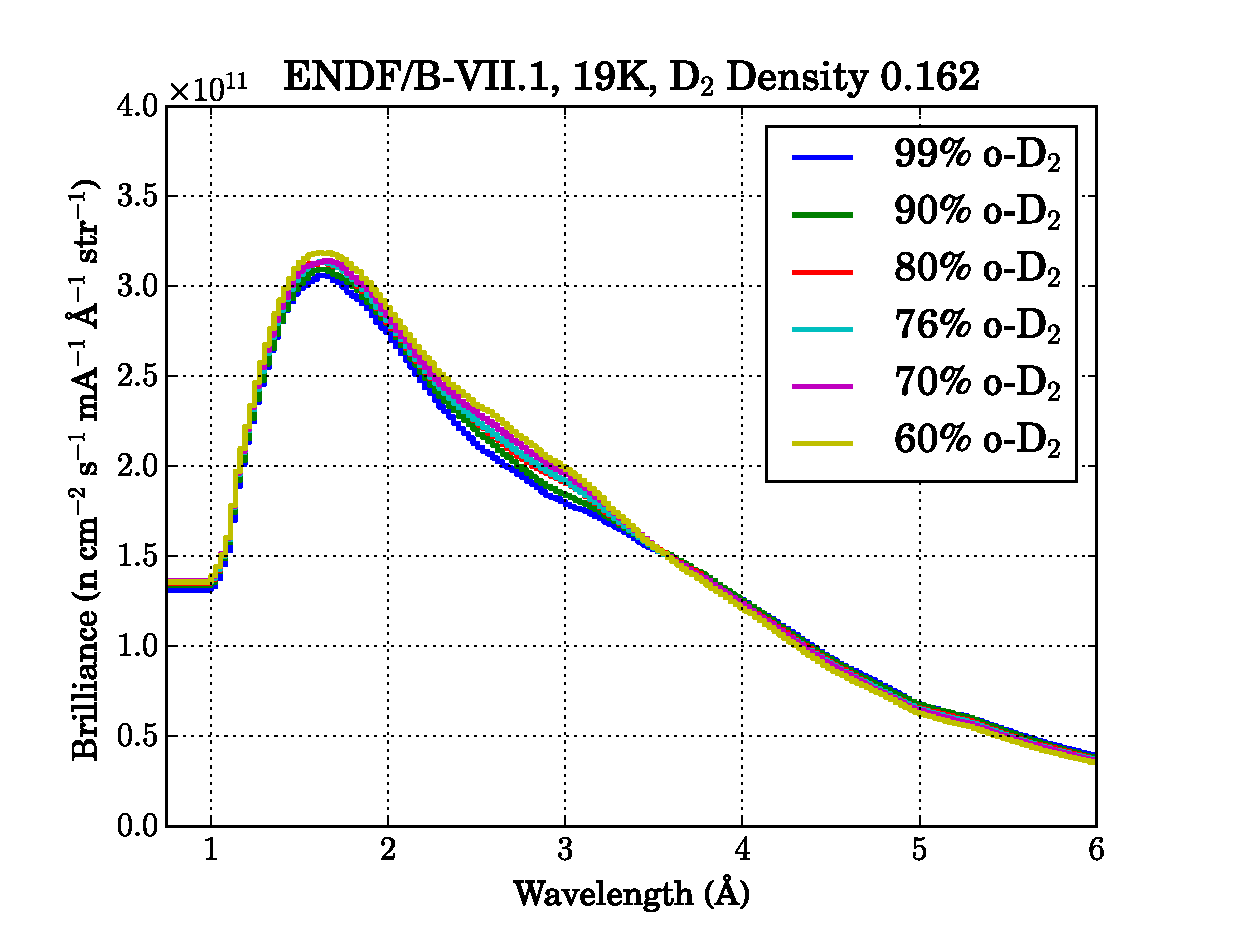
\includegraphics[width=\columnwidth]{graphics/op_compare.eps}
     \caption{Simulated neutron spectra emitted from liquid deuterium cold source at various ortho/para-D$_2$ ratios. ENDFB/VII.1 19 K scattering data and a D$_2$ density of 0.162 was used.   \label{fig:op_compare}}
\end{figure}

%
%
%
%
%

\section{Measured Brilliance and Best Matching Case}
\label{sec:results}

As mentioned previously, the state of the deuterium was uncertain due to the uncertainty in the irradiation history of the source (o/p fraction) and the total power deposited in the deuterium (density), but using the best information available, the most accurate results should comes from a simulation using the 24 K thermal scattering data from IKE and using an ortho-D$_2$ ratio of 0.761.  The beam current during the measurement was approximately 150 $\mu$A, so the power deposition inside the D$_2$ volume should have been approximately 75 Watts \cite{sinq_power}.  Therefore, based on previous studies on the void fraction in liquid D$_2$ under irradiation \cite{Siegwarth_Olson_Lewis_Rowe_Williams_1994}, the density should be near 98\% of the saturation density.  Figure \ref{fig:brilliance} shows the measured neutron spectra compared to simulated spectra at 98\% and 80\% saturation density, which are both included to show the most realistic case and the case which matches the peak intensity.  It is doubtful that the cold source had 20\% void during the measurement due to the low proton current, and was not considered to be a source of uncertainty in the final results.  An ortho fraction within the 60-99.5\% range, however, was considered to contribute to the uncertainty in the simulated results since the parameters entered into the fraction calculation were approximations (especially the catylitic conversion paramter). 

\begin{figure}[h!] 
  \centering
    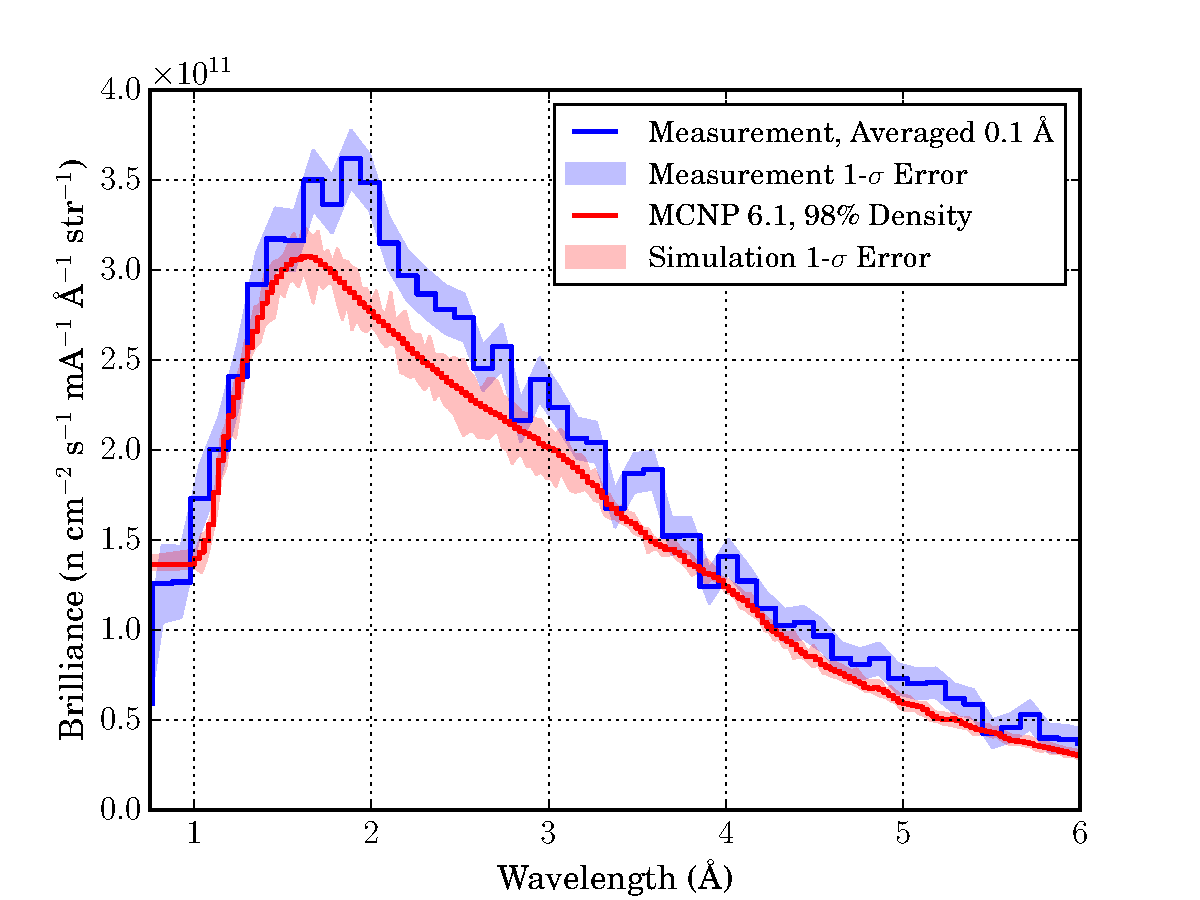
\includegraphics[width=\columnwidth]{graphics/brightness.pdf}
     \caption{Measured and simulated cold neutron source brilliance at the ICON beamline.  IKE 24 K scattering data and a o-D$_2$ fraction of 0.762 was used. \label{fig:brilliance} }
\end{figure}

Figure \ref{fig:brilliance} also shows that the peaks of simulated spectra are shifted about 0.25 {\AA} shorter with respect to the peak of the measured spectrum.  This phenomenon has been document previously, and it is suspected that it arises from some inaccuracies in the liquid deuterium thermal scattering data \cite{giller_thesis}.  The uncertainty in the distance between the chopper and the detector is approximately 10 cm, which corresponds to an uncertainty in the wavelength calibration of $\pm$ 0.3 {\AA}.  This value was calculated by propagating the positioning uncertainty through height between the bottom/top at the beryllium cut off wavelength and the moving average (smoothing) wavelength width (all of which were included in the uncertainty of the measurement).  

%
%
%
%
%

\section{Conclusions}
\label{sec:conclusions}

There are uncertainties associated with the state of the deuterium during the measurement, but reasonable attempts have been made to reduce or bound them where possible.  An approximate radiation-adjusted ortho-D$_2$ fraction was calculated using the proton beam history from the weeks leading up to the measurement time, the void fraction due to radiation heating was approximated, and appropriate scattering kernels for the deuterium temperature were used.  A measurement to determine the efficiency of the $^3$He detector was also done, the results of which match very well with MCNP simulation results.

The 0.25 {\AA} wavelength shift seen at the spectrum peak is within the positioning uncertainty of the measurement, and further conclusions about it cannot be made at this point.  The total view of the detector system was calculated to be $2.1363\times10^{-5}$ steradians via a MCNP calculation using a pinhole radiography tally.  The peak brilliance of the deuterium cold source at SINQ has been measured to be $3.5\times10^{11}$ n cm$^{-2}$ s$^{-1}$ mA$^{-1}$ \AA$^{-1}$ str$^{-1}$  $\pm$ $2.8\times10^{10}$ (8\%) at 1.9 {\AA} via a time-of-flight measurement at the ICON beamline in July 2014.  The total brilliance (energy-integrated) has been measured to be  $9.91\times10^{11}$  n cm$^{-2}$ s$^{-1}$ mA$^{-1}$ str$^{-1}$ $\pm$ $2.2\times10^{11}$ (23\%) for wavelengths above 0.7 {\AA}.  The simulated spectrum from the most probable state of the deuterium is within 20\% of the measured spectrum at ICON, which validates the MCNP model being used and sets a benchmark for future upgrade to be compared against.  

%
%
%
%
%

\section*{Acknowledgements}
\label{sec:ack}

This work was supported by Swiss National Science Foundation grant 200021\_150048/1.  A very special thank you to Wolfgang Bernnat as well as the Centro At\'{o}mico Bariloche team for providing the thermal cross section data, to Yong Dai for providing the STIP material compositions, and Anders Kaestner for all the help he provided on the ICON beamline.

%
%
%
%
%

\section*{References}
\bibliographystyle{elsarticle-num-names.bst}
\bibliography{brightness_manuscript}

\end{document}
